\documentclass[titlepage = firstcover]{scrartcl}
\usepackage[aux]{rerunfilecheck}
\usepackage{fontspec}
\usepackage[main=ngerman, english, french]{babel}

% mehr Pakete hier
\usepackage{expl3}
\usepackage{xparse}
\usepackage{pdfpages}

%Mathematik------------------------------------------------------
\usepackage{amsmath}   % unverzichtbare Mathe-Befehle
\usepackage{amssymb}   % viele Mathe-Symbole
\usepackage{mathtools} % Erweiterungen für amsmath
\usepackage[
  math-style=ISO,    % \
  bold-style=ISO,    % |
  sans-style=italic, % | ISO-Standard folgen
  nabla=upright,     % |
  partial=upright,   % /
]{unicode-math}% "Does exactly what it says on the tin."

% Laden von OTF-Mathefonts
% Ermöglich Unicode Eingabe von Zeichen: α statt \alpha

\setmathfont{Latin Modern Math}
%\setmathfont{Tex Gyre Pagella Math} % alternativ zu Latin Modern Math
\setmathfont{XITS Math}[range={scr, bfscr}]
\setmathfont{XITS Math}[range={cal, bfcal}, StylisticSet=1]

\AtBeginDocument{ % wird bei \begin{document}
  % werden sonst wieder von unicode-math überschrieben
  \RenewDocumentCommand \Re {} {\operatorname{Re}}
  \RenewDocumentCommand \Im {} {\operatorname{Im}}
}
\usepackage{mleftright}
\setlength{\delimitershortfall}{-1sp}

%Sprache----------------------------------------------------------
\usepackage{microtype}
\usepackage{xfrac}
\usepackage[autostyle]{csquotes}    % babel
\usepackage[unicode, pdfusetitle]{hyperref}
\usepackage{bookmark}
\usepackage[shortcuts]{extdash}
%Einstellungen hier, z.B. Fonts
\usepackage{booktabs} % Tabellen
\usepackage{a4}
\usepackage{float}

\setlength{\parindent}{0pt}


\title{Fourier-Synthese}
\author{David Gutnikov \and Lasse Sternemann}
\date{Durchführung am 5.11.19}


\begin{document}

    \maketitle
    \tableofcontents
    \newpage

    \section{Theorie der Fourier-Synthese}
    Mit dem mathematischen Konzept der Fourier-Synthese kann man jede periodische Funktion durch eine Addition
    von Sinus- und Kosinusfunktionen darstellen. 
    \begin{align}
        f(t) &= \sum_{k=0}^\infty (A_k cos(\omega_k t)+B_k sin(\omega_k t))  & mit\; \omega_k &= \frac{2 \pi k}{T} 
    \end{align}
    Die Koeffizienten aus Formel (1) lassen sich wie folgt bestimmen.
    \begin{align*}
        A_k &= \frac{2}{T} \int_{-\frac{T}{2}}^{\frac{T}{2}} f(t) cos(w_k t)dt  & mit\; A_0 &= \frac{1}{T} \int_{-\frac{T}{2}}^{\frac{T}{2}} f(t)dt   \vspace{80pt}        \\ 
        B_k &= \frac{2}{T} \int_{-\frac{T}{2}}^{\frac{T}{2}} f(t) sin(w_k t)dt   & mit\; B_0 &= 0 
    \end{align*}
    Wenn die Funktion eine Symmetrie aufweist, kann die Synthese vereinfacht werden. So müssen bei punktsymmetrischen/ungeraden Funktionen
    die Kosinus-Terme wegfallen und $A_k$ wird gleich Null gesetzt. Wenn die Funktion achsensymmetrisch/gerade ist, wird  der Sinus weggelassen und
    und demenstprechend $B_k$ gleich Null gesetzt.

    \section{Fourier-Synthese von $f(t)=|sin(t)|$}
    Die anzunähernde Funktion ist achsensymmetrisch/gerade und $B_k$ wird daher gleich Null gesetzt. Es wird eine Periode $T=\pi$ gewählt 
    und die Frequenz $\omega_k$ entspricht demnach $2k$. 
    \begin{equation}
        f(t) = \sum_{k=0}^{17} (A_k cos(\omega_k t))
    \end{equation} 
    Formel (2) ist die zu bestimmende Funktion. Nun müssen noch die Koeffizienten $A_0$ bis $A_{17}$ mit einem Python Programm bestimmt werden.
    \begin{gather*}
        A_0 = \frac{1}{T} \int_{-\frac{T}{2}}^{\frac{T}{2}} |sin(t)|dt \\
        A_k = \frac{2}{T} \int_{-\frac{T}{2}}^{\frac{T}{2}} |sin(t)| cos(w_k t)dt 
    \end{gather*}
    \newpage
    Aus den Berechnungen ergibt sich das Frequenzspektrum (Tabelle 1 und Abbildung 1) und die angenäherte Funktion (Abbildung 2).

    \begin{table}[h]
        \centering
        \caption{Frequenzspektrum}
        \label{tab:Tabelle_1}
        
        \begin{tabular}{c c}
            \toprule
            {$k = \frac{\omega_k}{2}$} & {$A_k$}\\
            \midrule
            0 &  0,0000 \\
            1 & 2,0000  \\
            2 & -1,0000 \\
            3 & 0,6667  \\
            4 & -0,5000 \\
            5 & 0,4000  \\
            6 & -0,3334 \\
            7 & 0,2857  \\
            8 & -0,2500 \\
            9 & 0,2223  \\
            10 & -0,2000    \\
            11 & 0,1818 \\
            12 & -0,1667 \\
            13 & 0,1538 \\
            14 & -0,1429 \\
            15 & 0,1334 \\
            16 & -0,1250 \\
            17 & 0,1176 \\
            \bottomrule
        \end{tabular}    
    \end{table}

    \begin{figure}[H]
        \centering
        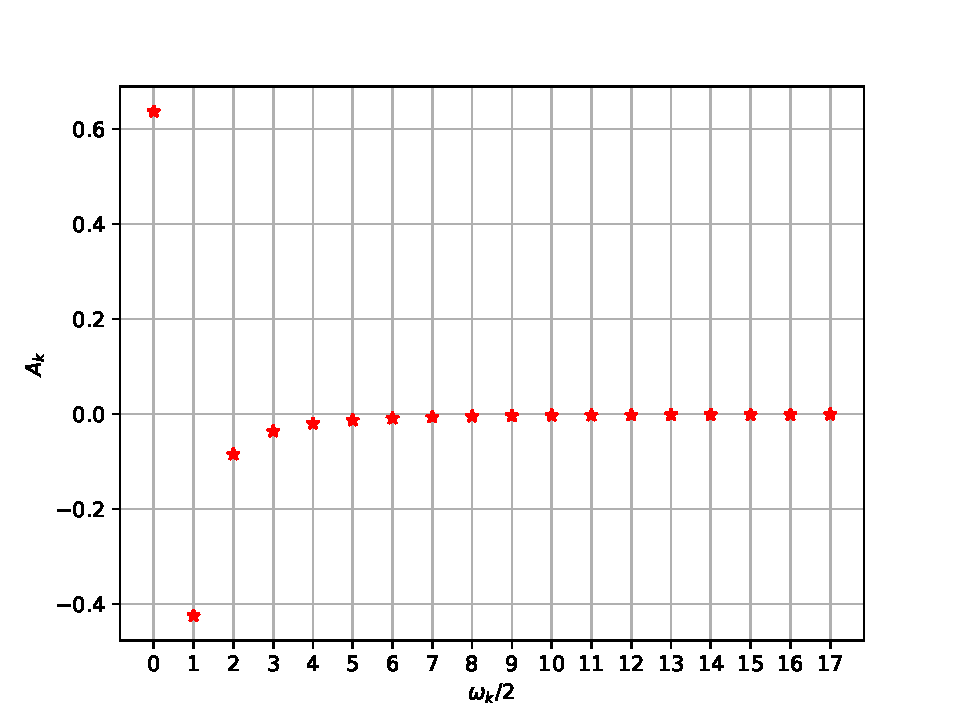
\includegraphics[width=0.9\linewidth]{Freqspek_y=|sin(x)|.pdf}
        \caption{Frequenzspektrum der Fourier-Synthese von $f(t)=|sin(t)|$}
    \end{figure}
    \begin{figure}[H]
        \centering
        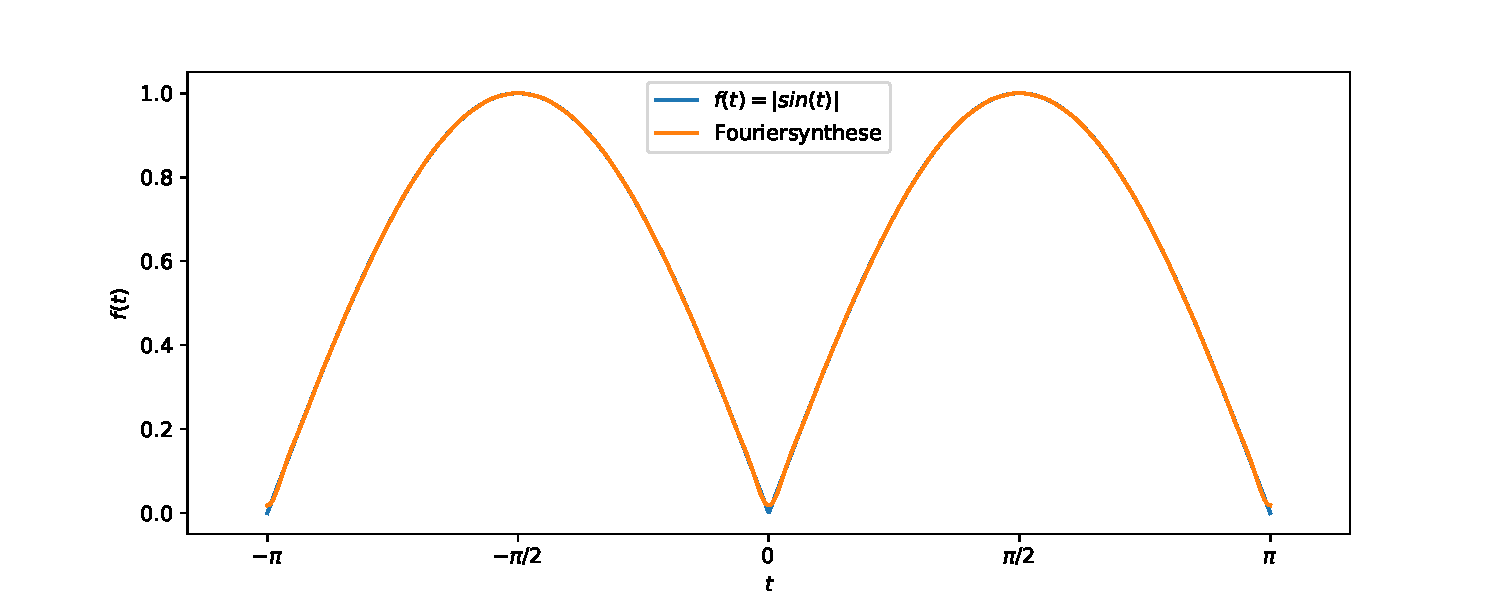
\includegraphics[width=1.2\linewidth]{plot_sin.pdf}
        \vspace{-5mm}
        \caption{Graph der Fourier-Synthese von $f(t)=|sin(t)|$}
    \end{figure}



    \section{Fourier-Synthese von $f(t)=t$}
    Die anzunähernde Funktion ist punktsymmetrisch/ungerade und $A_k$ wird daher gleich Null gesetzt. Es wird eine Periode $T=2\pi$ gewählt 
    und die Frequenz $\omega_k$ entspricht demnach $k$.
    \begin{equation}
        f(t) = \sum_{k=0}^{17} B_k sin(\omega_k t)
    \end{equation} 
    Formel (3) ist die zu bestimmende Funktion. Nun sind noch die Koeffizienten $B_0$ bis $B_{17}$ mit einem Python Programm zu bestimmen.
    \begin{gather*}
        B_0 = 0 \\
        B_k = \frac{2}{T} \int_{-\frac{T}{2}}^{\frac{T}{2}} t sin(w_k t)dt \\
    \end{gather*}
    Aus den Berechnungen ergibt sich das Frequenzspektrum (Tabelle 2 und Abbildung 3) und die angenäherte Funktion (Abbildung 4).
    
    \begin{table}[h]
        \centering
        \caption{Frequenzspektrum}
        \label{tab:Tabelle_2}
        
        \begin{tabular}{c c}
            \toprule
            {$k = \omega_k$} & {$B_k$}\\
            \midrule
            0 &  0,6366 \\
            1 & -0,4244 \\
            2 & -0,0849 \\
            3 & -0,0364 \\
            4 & -0,0202 \\
            5 & -0,0129 \\
            6 & -0,0089 \\
            7 & -0,0065 \\
            8 & -0,0050 \\
            9 & -0,0039 \\
            10 & -0,0032 \\
            11 & -0,0026 \\
            12 & -0,0022 \\
            13 & -0,0019 \\
            14 & -0,0016 \\
            15 & -0,0014 \\
            16 & -0,0012 \\
            17 & -0,0011 \\
            \bottomrule
        \end{tabular}    
    \end{table}
    
    \begin{figure}[H]
        \centering
        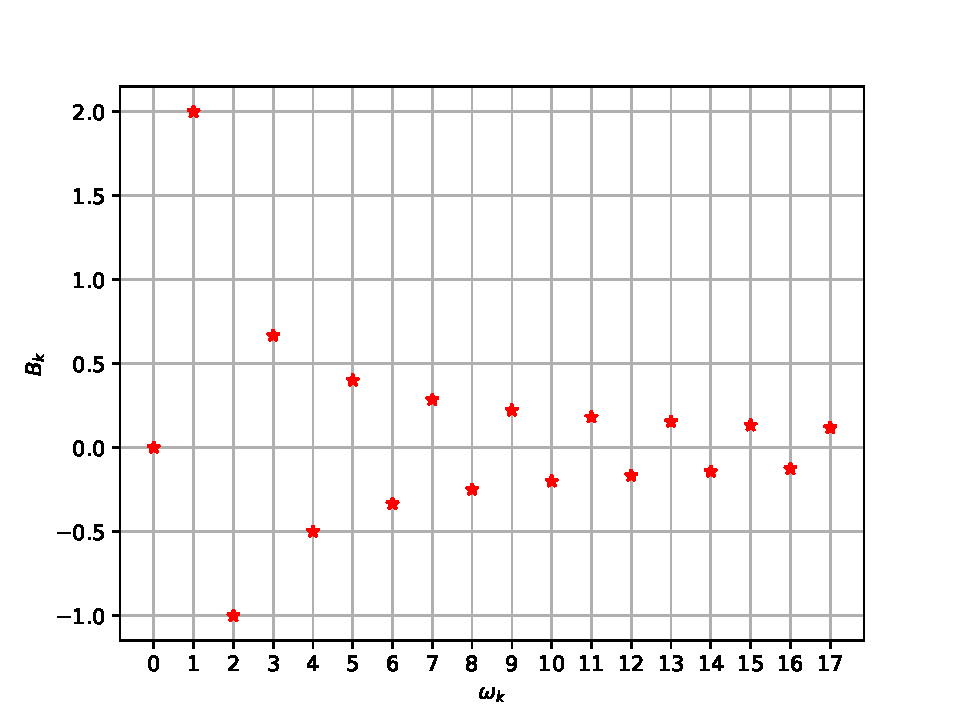
\includegraphics[width=0.9\linewidth]{Freqspek_y=x.pdf}
        \vspace{-5mm}
        \caption{Frequenzspektrum der Fourier-Synthese von $f(t)=t$}
    \end{figure}
    \begin{figure}[H]
        \centering
        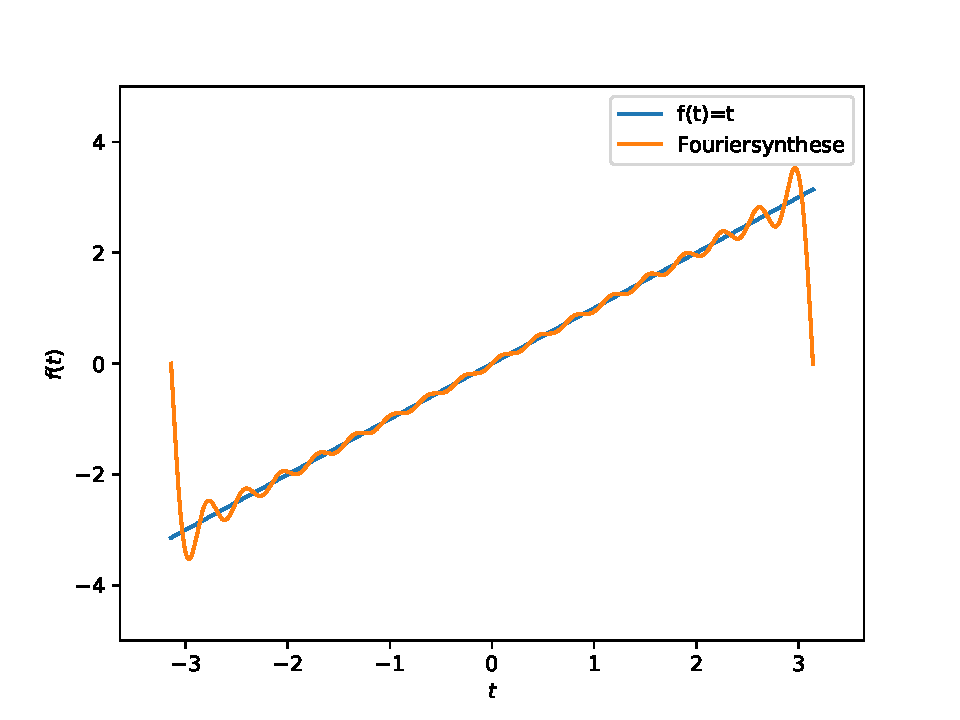
\includegraphics[width=1.2\linewidth]{plot_x.pdf}
        \vspace{-10mm}
        \caption{Graph der Fourier-Synthese von $f(t)=t$}
    \end{figure}


\end{document}

